\section{Evaluation}
\label{sec:Eval}

We focus our evaluation on two major aspects of \emph{PostBOUND}: On the one hand, we examine the independence of \emph{PostBOUND} from specific workloads using two well-known benchmarks and different PostgreSQL versions.
On the other hand, we explore the potential of upper bound-driven query optimization in more detail.
This includes (i) the computed join orders, (ii) the generation of subqueries, (iii) the effect of tighter upper bounds, and (iv) the potential of the selection of physical operators.
Generally, all experiments are executed on an Ubuntu 20.04 machine with an Intel i7-6700 HQ processor, 32 GB of main memory and an SSD storage.
Unless stated otherwise, we run the benchmarks on PostgreSQL 14.

%\subsection{Analyzing UES: Join Orders and Subquery Generation}
%\label{sec:eval-postbound}

\textbf{Analyzing UES - Join Orders:}
To analyze \emph{PostBOUND}s applicability to different database schemas and workloads, we examined the Join-Order-Benchmark (JOB)~\cite{DBLP:journals/pvldb/LeisGMBK015} as well as the Star-Schema-Benchmark (SSB)~\cite{DBLP:journals/corr/Sanchez16a}. 
Queries of the JOB are optimized with UES using the precise base table estimation and defensive subquery generation strategies (cf. Section~\ref{sec:postbound-join-ordering}). 
Precise base table estimation allows for the best reproducibility of the optimized queries, since the estimates are derived directly from the live database. 
Moreover, the defensive subquery generation was also used in \cite{hertzschuch-21-ues} enabling better comparability with these results. 
The queries of the SSB are optimized based on the base table estimates of the native PostgreSQL optimizer to demonstrate this functionality. 
The underlying TPC-H database is setup to use a scale factor of $1$. 
In addition to different benchmarks, we also evaluate both workloads on two versions of PostgreSQL: v12.4 was already used in \cite{hertzschuch-21-ues} and v14.2 is the latest release of PostgreSQL at the time initial work on \emph{PostBOUND} began. Table~\ref{tab:postbound-benchmarks} contains the total runtime for each benchmark setting. 
Native optimization in this context means optimization by the built-in optimizer of PostgreSQL, but without usage of nested loop joins.  
This constraint matches a similar requirement by UES and fits our focus on the resulting join orders for this experiment, since UES only uses hash-joins.

\begin{table}[t]
    \centering
    \begin{tabular}{|c||c|c||c|c|}
        \hline
         Benchmark& \multicolumn{2}{c||}{PostgreSQL v12.4} & \multicolumn{2}{c|}{PostgreSQL v14.2} \\
         & Native & UES & Native & UES \\
         \hline
         Join-Order-Benchmark (JOB) & 535.2s & 399.5s & 359.4s & 377.0s \\
         Star-Schema-Bechmark (SSB) & 5.1s & 5.5s & 5.1s & 5.3s \\
         \hline
    \end{tabular}
    \caption{Total runtimes of different benchmarks using different PostgreSQL versions.}
    \label{tab:postbound-benchmarks}
    \vspace{-0.4cm}
\end{table}

The JOB benchmark results highlights two interesting insights: On the one hand, using PostgreSQL v12.4 shows a much better performance of UES compared to the native optimizer.
This basically confirms the results presented in \cite{hertzschuch-21-ues}. 
On the other hand, PostgreSQL v14.2 has a slightly better runtime than its UES counterpart. 
This demonstrates the significantly improved join ordering of PostgreSQL during the last two major releases: As long as no regressions occur, a traditional optimizer can produce more aggressive plans, which UES avoids due to their bad worst-case cardinality. 
If this worst case does not come to pass, UES can be too defensive. 
For example, this situation occurs in 6 queries that together amount to about 17 seconds of native speedup. 
Calculating tighter upper bounds may prevent such behavior.
Results on SSB are much more similar, which is mostly caused by the much smaller data set. However, the runtimes show that the UES optimized queries are neither significantly better, nor significantly worse than native optimization. 
Nonetheless, the overall simpler queries of the SSB also stray away from the primary focus of upper bound-driven query optimization, which is intended for complex queries with many joins and complicated filter predicates.

\begin{figure}[tb]
	\centering
	\begin{subfigure}[b]{0.47\textwidth}
	    \centering
	    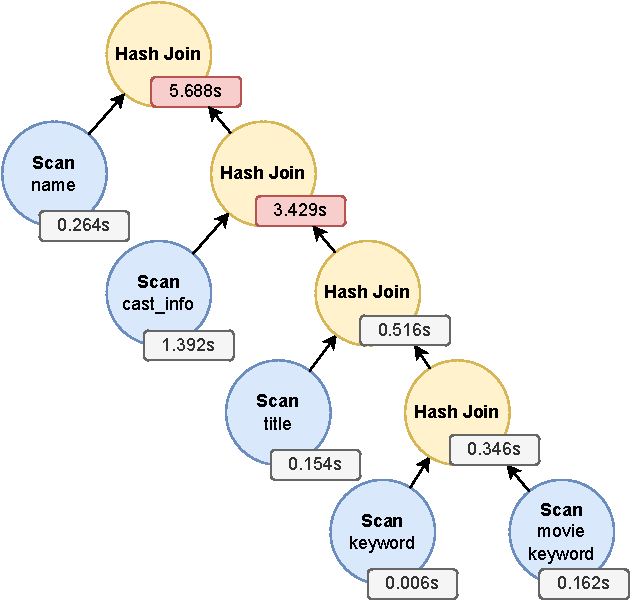
\includegraphics[width=0.8\textwidth]{figures/subquery-example-job-6c-linear.pdf}
	    \caption{Linear execution plan.}
	    \label{fig:subquery-results-linear}
	\end{subfigure}
	\begin{subfigure}[b]{0.47\textwidth}
	    \centering
	    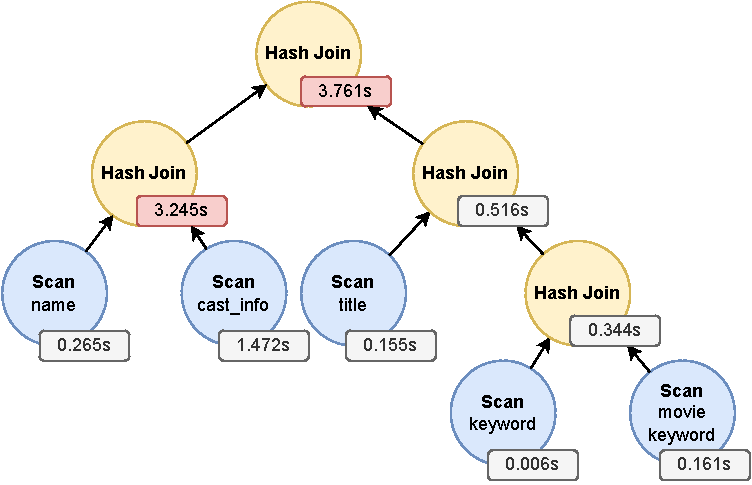
\includegraphics[width=\textwidth]{figures/subquery-example-job-6c-subqueries.pdf}
	    \caption{Bushy execution plan}
	    \label{fig:subquery-results-bushy}
	\end{subfigure}
	\caption{Generating subqueries for JOB query 6c can improve performance substantially.}
	\label{fig:subquery-results}
	\vspace{-0.4cm}
\end{figure}

\textbf{Analyzing UES - Subquery Generation:}
A central idea of UES is the evaluation of primary key/foreign key joins in subqueries to achieve an up-front reduction of the foreign key cardinality. 
However, introducing subqueries also implies additional pipeline breakers during query execution. 
Thus, we investigate the impact of subqueries on individual queries next by optimizing the JOB workload with two UES settings: The first one uses the smart subquery generation strategy while the second setting produces entirely linear queries.
Based on this setup, for example, query 6c shows the largest speedup of about 33\% (5.7s to 3.8s) when using subqueries. 
The resulting execution plans for both settings are sketched in Fig.~\ref{fig:subquery-results}: executing the join between \sql{name} and \sql{cast\_info} as a subquery not only reduces the number of processed tuples, but also allows for a parallel processing of that join. 
Nevertheless, subqueries do not always lead to a performance benefit. 
In fact, query 7a is slowed down the most with about 0.6 seconds (13\% of the linear runtime). 
Thus, it is important to create subqueries carefully and a smart generation policy, e.g., based on tight upper bounds seems to work well in these cases.

%\subsection{Advancing UES: Tighter bounds and physical operators}
%\label{sec:eval-tighter-bounds}


\textbf{Advancing UES - Tighter Upper Bounds:}
Tight upper bounds have been proposed as a potential solution for many problems in this paper. 
In this section, we evaluate how large the impact of the cautious and approximate algorithms presented in Section~\ref{sec:TighterBounds} already is. 
For this, we vary the length of the top-k lists for both algorithms and compare the results to a UES baseline. 
In all cases, the JOB queries are upper bound-driven optimized using precise base table estimates and the smart subquery generation policy.

Looking at the median upper bounds across all JOB queries in Fig.~\ref{fig:results-topk-upper-bounds} indeed reveals a substantial improvement of the bounds as the top-k lists become longer.
In fact, using top-500 lists achieves a maximum improvement of factor 210,000 compared to the UES bound. 
Although this is an extreme case, many upper bounds still improve several orders of magnitude when using top-k lists with just 50 or 100 attribute values. 
For shorter top-k lists, the improvement is much smaller, as is expected. 
This is caused by two main factors: shorter lists allow for fewer actual matches of attribute values, causing more usage of the $f^\ast$ frequencies.
At the same time, shorter lists also allow for less drop-off of frequencies, again resulting in values that are closer to the UES bound.

\begin{figure}[tb]
	\centering
	\begin{subfigure}[b]{0.47\textwidth}
	    \centering
	    \includegraphics[width=\textwidth]{figures/plot-job-upper-bounds.pdf}
	    \caption{Final bounds of each query.}
	    \label{fig:results-topk-upper-bounds}
	\end{subfigure}
	\begin{subfigure}[b]{0.47\textwidth}
	    \centering
	    \includegraphics[width=\textwidth]{figures/plot-job-optimization-time.pdf}
	    \caption{Optimization time of the workloads.}
	    \label{fig:results-topk-optimization-time}
	\end{subfigure}
	\caption{Impact of the top-k based bound estimation on the JOB queries.}
	\label{fig:results-topk}
	\vspace{-0.4cm}
\end{figure}

A central advantage of the approximate formula becomes apparent when looking at the optimization time in Fig.~\ref{fig:results-topk-optimization-time}: It stays very low at a maximum of 3 seconds for all queries in the JOB. 
This is a sharp contrast to the cautious formula, that takes over 1 minute of optimization time already at top-5 lists. 
This increase in optimization time is also the reason why larger top-k lists are not optimized with the naive implementation of the algorithm.
Despite the smaller bounds, only a few join orders are actually updated. 
In fact, the cautious algorithm only updates 5 queries across all settings. 
Although this number becomes slightly larger with 31 queries for the approximate formula, it is still quite small considering the 113 queries that are executed. 
This indicates that UES is sufficient for many queries and that more elaborate algorithms are required to close in on the estimates of the native optimizer. 
The few updated queries also lead to very little change of the overall workload runtime. 
Across all settings, the maximum deviation from UES is about 10 seconds, which is almost negligible considering the complexity of the workload and its overall duration.
Even though the evaluated formulas are prototypes by nature, they still achieve a considerable improvement in terms of their upper bounds. 
This motivates further research in that direction and especially the application of the bounds for different tasks.

\begin{figure}[tb]
	\centering
	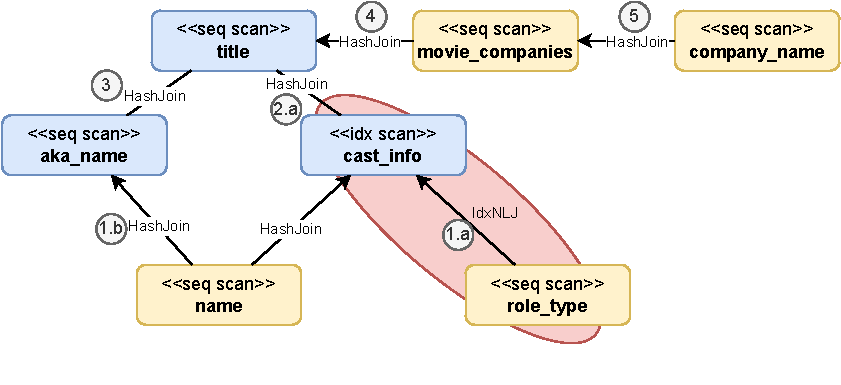
\includegraphics[width=0.95\linewidth]{figures/idxnlj-example-job-8d.pdf}
	\caption{Join order and operator selection for JOB query 8d. Subqueries use Index-NLJ hints.}
	\label{fig:idxnlj-results}
	\vspace{-0.4cm}
\end{figure}

\textbf{Advancing UES - Physical Operator Selection:}
Besides the generation of optimized join orders, \emph{PostBOUND} also enables the selection of physical operators (cf. Section~\ref{sec:postbound-operator-selection}), thereby removing the restriction to hash joins normally imposed by UES. 
A natural application of the operator selection is to further exploit the performance gains enabled by subqueries. 
Since these queries are by design joins between a primary key and a foreign key table, they can be implemented efficiently using index-nested loop joins. 
Thus, we again optimize the JOB workload using UES and the smart subquery generation policy. 
For each resulting subquery, we use \emph{PostBOUND} to generate query hints that enforce the execution of that subquery as an index-nested loop join. Fig.~\ref{fig:idxnlj-results} shows the final execution plan for query 8d, which is improved the most by this strategy. 
Primary key filters are shown in yellow boxes while tables that are n:m joined appear in blue. 
Each join is annotated by its operator, as well as the point in time when it is executed. 
The subquery \sql{cast\_info $\bowtie$ role\_type} is executed as an index-nested loop join in parallel to the join \sql{aka\_name $\bowtie$ name}. 
The choice of operators results in a 45\% speedup (5.7s to 2.6s) compared to a pure hash join-based execution. 
This simple strategy barely scratches the surface of elaborate techniques for physical operator selection, it focuses exclusively on joins between base tables within subqueries and does not consider the upper bounds associated with each join at all. 
Advanced approaches such as TONIC~\cite{DBLP:journals/pvldb/HertzschuchHHL22} could perform much better. 
Still, the simple strategy of executing all subqueries as index-nested loop joins already shows the potential of appropriate operator choice that can be explored in future work.
